\documentclass[12pt]{article}
\usepackage{amsmath, amssymb, amsfonts, bm, graphicx, geometry, tabularx, booktabs, float, enumitem,cancel}
\geometry{margin=1in}

\title{ESC 330 Exam 1 Resub (Problem 2)}
\date{}
\author{}

% Uppercase Volume with thicker, higher line
\newcommand{\vol}{\mathord{\text{\ooalign{\hidewidth $V$\hidewidth\cr\kern-0.5pt\raisebox{0.8ex}{\rule[0pt]{1em}{0.5pt}}}}}}

% Lowercase Volume with built-in shifts
\newcommand{\svol}{%
  \mathord{\text{\ooalign{%
    \hfil$v$\hfil\cr
    \hfil\rule[0.6ex]{0.8em}{0.5pt}\hfil
  }}}%
}

\begin{document}
\maketitle
\vspace{-5em}
\begin{center}
    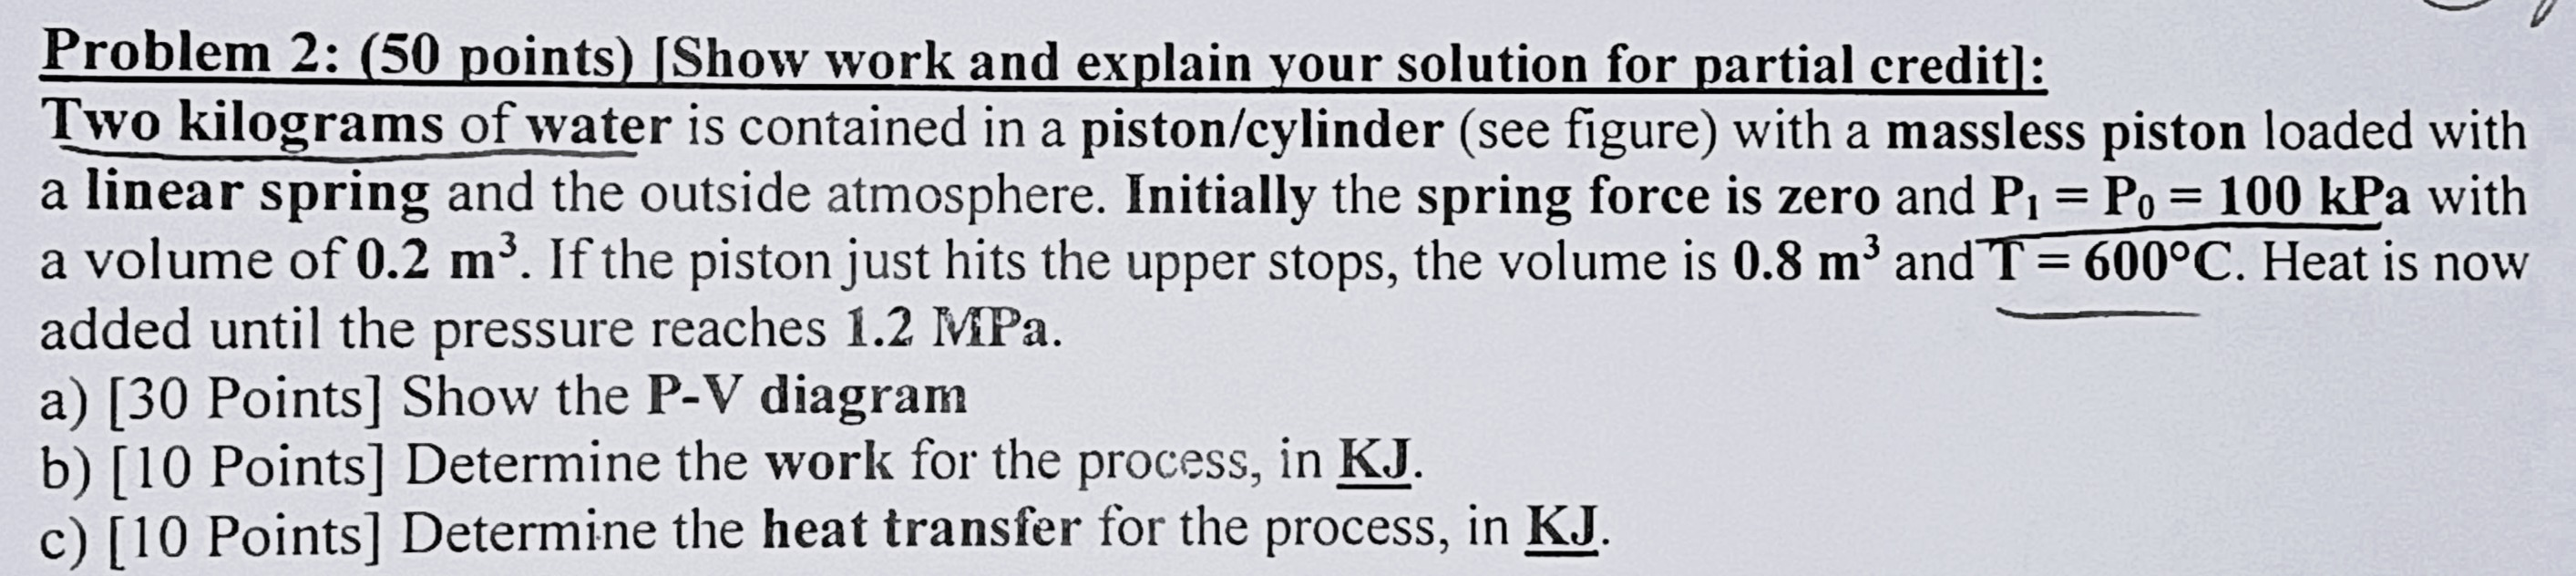
\includegraphics[width=1\textwidth]{P2.jpg}
\end{center}
\begin{center}
    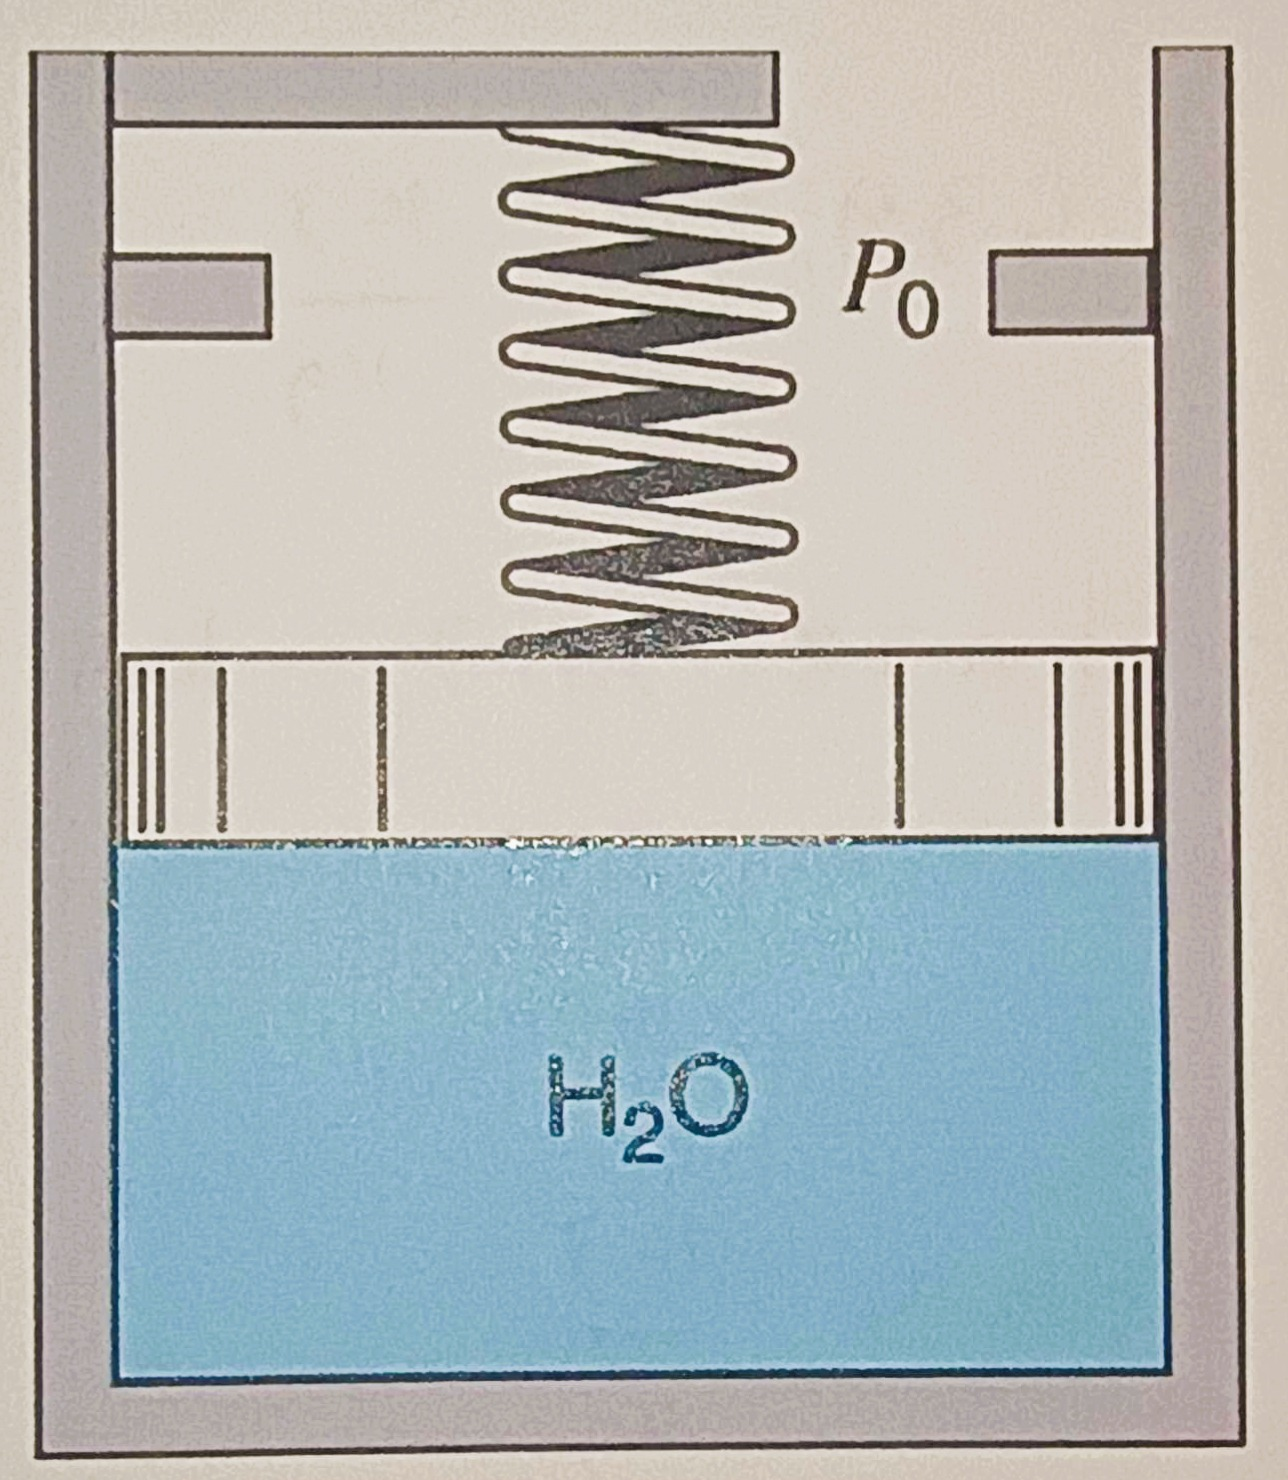
\includegraphics[width=0.3\textwidth]{P2-1.jpg}
\end{center}
\begin{enumerate}
    \item \textbf{Objective:}
    \begin{itemize}
        \item Show the P-$\vol$ diagram for the process.
        \item Find the work for the process $W$ [kJ].
        \item Find the amount of heat transfer for the process $Q$ [kJ].
    \end{itemize}
    \item \textbf{Schematic:}
    \begin{center}
        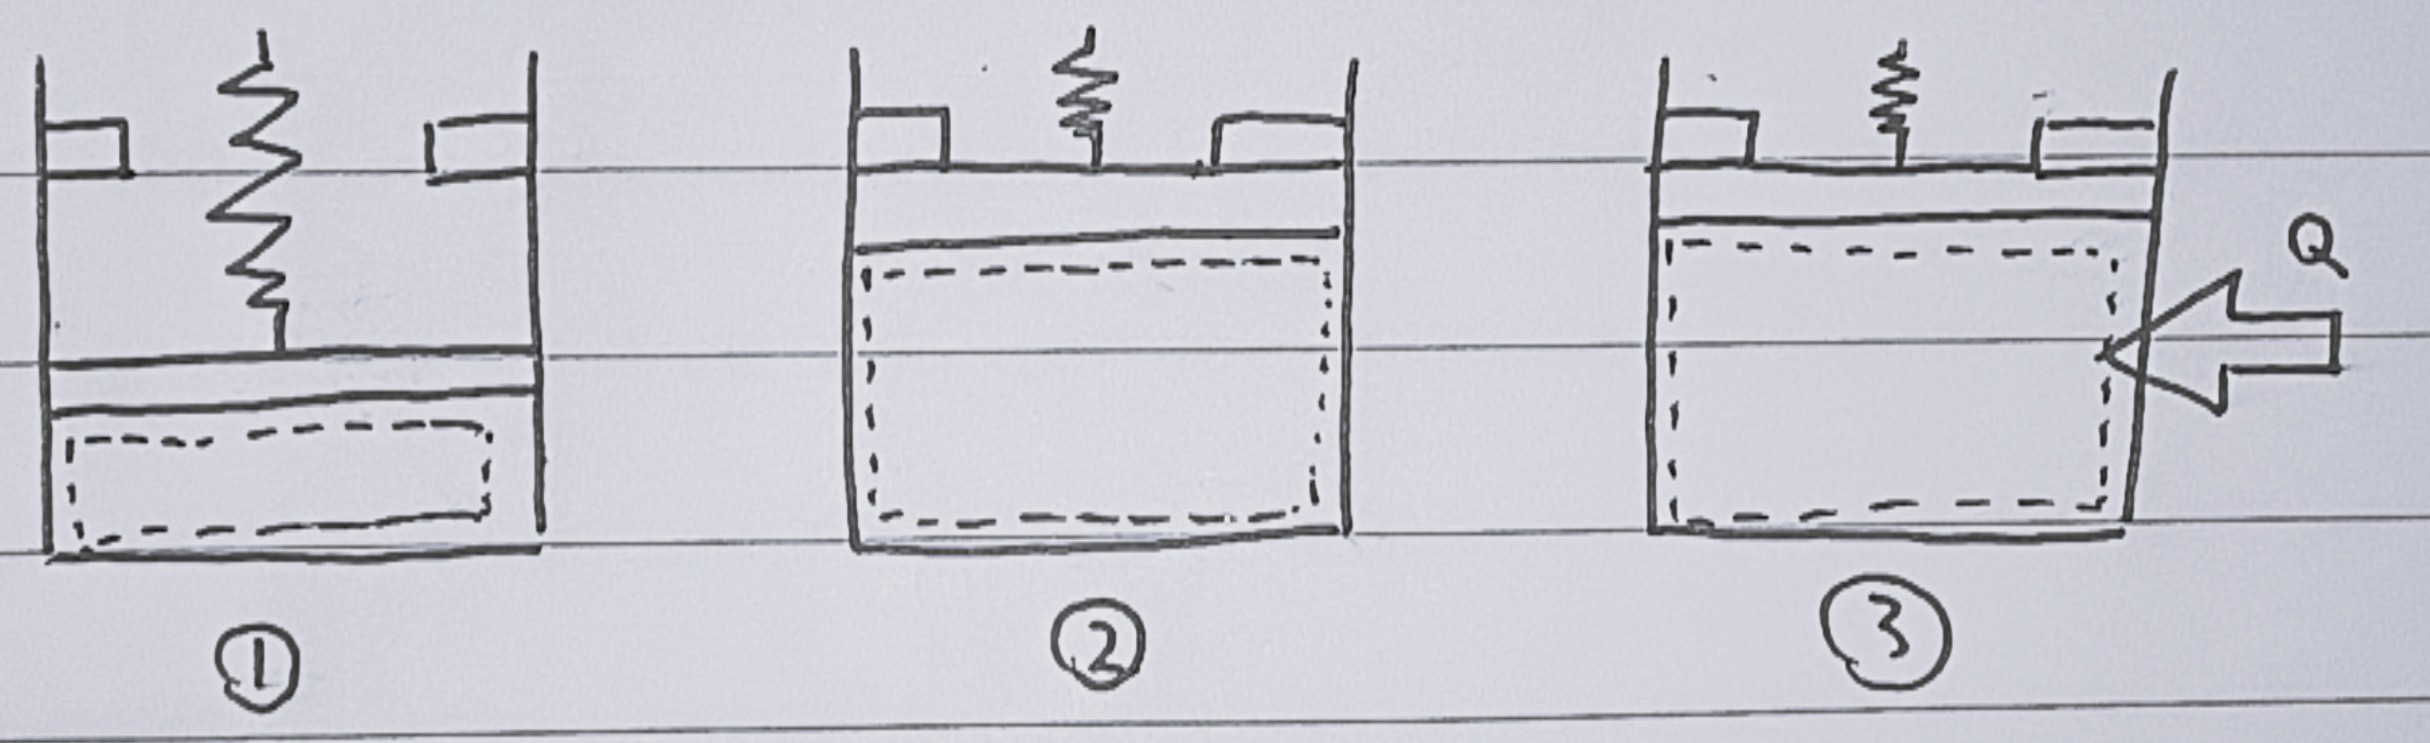
\includegraphics[width=0.8\textwidth]{Schem.jpg}
    \end{center}
    \newpage
    \item \textbf{Given:}
    \begin{itemize}
        \item \textit{Closed system}: containing $m= 2$ kg of \textit{water}.
        \item State 1: $P_1 = 100$ kPa, $\vol_1 = 0.2$ m$^3$ $\implies \svol_1 = 0.1$ m$^3$/kg 
        \item State 2: $\vol_2 = 0.8$ m$^3$, $T_2 = 600^\circ$C $\implies \svol_2 = 0.4$ m$^3$/kg
        \item State 3: $\vol_3 = 0.8$ m$^3$, $P_3 = 1.2$ MPa $\implies \svol_3 = 0.4$ m$^3$/kg
    \end{itemize}
    \item \textbf{Approach:}
    \begin{itemize}
        \item Use property tables to determine phases and properties for states 1-3 and plot them onto a P-$\vol$ diagram.
        \item Determine work of the process using the equation of work for a \textit{closed system}:
        \[W_\text{closed} = \int P\, d\vol = m\int P\,d\svol\]
        \item Apply the first law for a closed system to determine the heat transfer for the process $Q$:
        \[\Delta U = Q-W\]
    \end{itemize}
    \item \textbf{P-$\vol$ Diagram:}
    \begin{itemize}
        \item State 1: at $P_1 = 100$ kPa, $\svol_f < \svol_1 < \svol_g$ implies that state 1 is a \textit{saturated mixture}. Thus, its temperature is the saturation temperature at $P_1$, which is $T_1 = 99.61^\circ$C.
        \item State 2: at $T_2 = 600^\circ$C, it is a \textit{superheated vapor}. Looking at the superheated water tables, we find that for $T_2 = 600^\circ$C and $\svol_2 = 0.40111 \approx 0.4$ m$^3$/kg, the pressure is $P_2 = 1$ MPa.
        \item State 3: Since state 2 is a superheated vapor and heat is added from state 2 to state 3, state 3 must also be a superheated vapor. Since volume is constant from state 2 to state 3, we have $\svol_3 = \svol_2 = 0.4$ m$^3$/kg (isochoric process). We are given that $P_3 = 1.2$ MPa.
    \end{itemize}
    \vspace{-1em}
    \setlength{\fboxsep}{10pt} % adjust padding
    \begin{center}
        \fbox{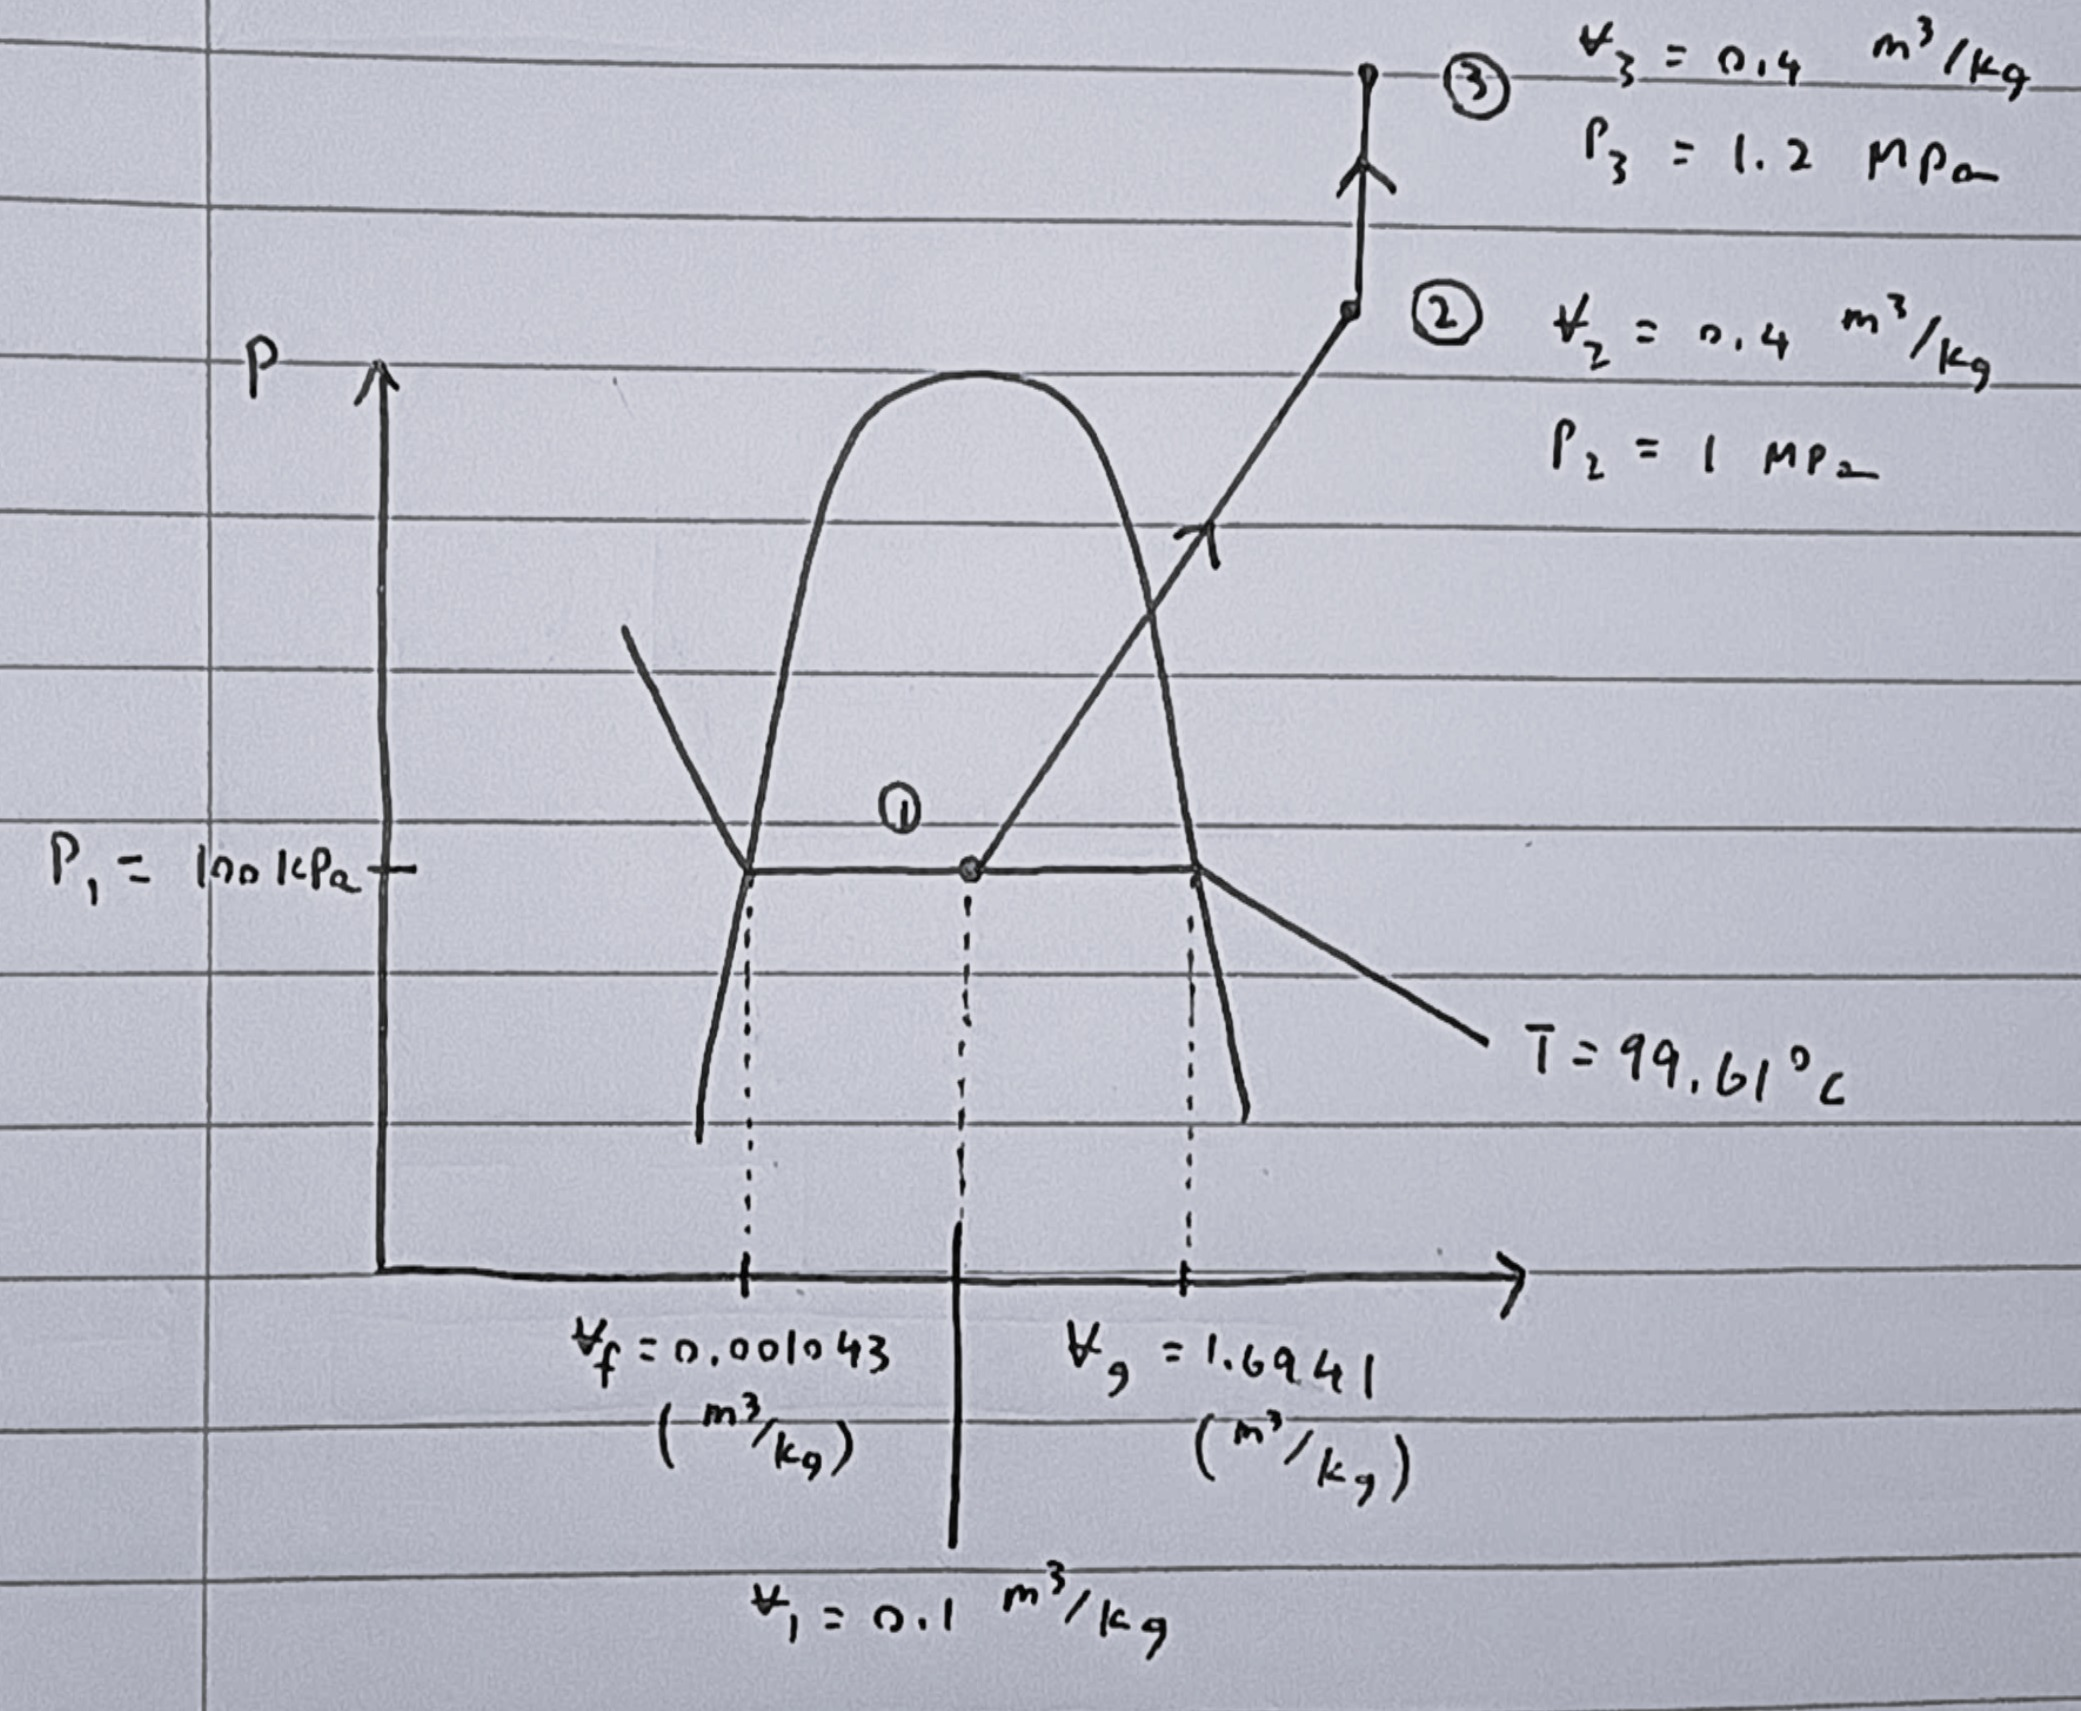
\includegraphics[width=0.8\textwidth]{PV.jpg}}
    \end{center}
    \item \textbf{Work of a closed system:}\\
    Since there is no change of volume from state 2 to state 3, there is no work done during this process. Thus, we only need to calculate the work done from state 1 to state 2:
    \[W_{1 \to 2 } = m\int_{\svol_1}^{\svol_2} P\,d\svol\]
    Geometrically, this is the area under the curve from state 1 to state 2 on the P-$\vol$ diagram. This is the same as the area of the trapezoid formed by states 1 and 2:
    \[\begin{aligned}
    W_{1 \to 2} &= m\left(\frac{P_1 + P_2}{2}\right)(\svol_2 - \svol_1)\\
    &= [2\,\text{kg}]\left(\frac{[100+1000\,\text{kPa}]}{2}\right)([0.4 - 0.1\,\text{m}^3/\text{kg}])\\
    &= 330\,\text{kJ}
    \end{aligned}\]
    \[\boxed{\implies W_{1\to3} = W_{1\to2}+\underbrace{\cancel{W_{2\to3}}}_{0}=330\,\text{kJ}}\]
\underline{Note:} A quicker way to approximate the work is to use a rectangular area using the average pressure $P_\text{avg} = (P_1 + P_2)/2$ and the change in volume $\Delta \vol = m(\svol_2 - \svol_1)$.
\newpage
    \item \textbf{Heat transfer:}\\
    Knowing work, we just need to use the property tables to find the specific internal energies at states 1 and 3:
    \begin{itemize}
        \item State 1:\\
        Since state 1 is a saturated mixture, we can find the quality $x_1$ using the specific volume:
        \[x_1 = \frac{\svol_1 -\svol_f}{\svol_g-\svol_f} = \frac{[0.1 - 0.001043\,\text{m}^3/\text{kg}]}{[1.6941 - 0.001043\,\text{m}^3/\text{kg}]} = 0.0584\]
        Use quality to find the specific internal energy at state 1:
        \[\begin{aligned}
        u_1 &= u_f + x_1u_{fg}\\
        &= [417.40\,\text{kJ/kg}] + 0.0584[2088.2\,\text{kJ/kg}] = 539.45\,\text{kJ/kg}
        \end{aligned}\]
        \item State 3:\\
        Linear interpolation for the superheated water tables at $P_3 = 1.2$ MPa, using the values at
        \begin{itemize}
            \item $T=700^\circ$C: $\svol = 0.37297$ m$^3$/kg, $u = 3475.3$ kJ/kg
            \item $T=800^\circ$C: $\svol = 0.41184$ m$^3$/kg, $u = 3661.0$ kJ/kg
        \end{itemize}
        \[\begin{aligned}
        u - u_{800} &= \frac{u_{800}-u_{700}}{\svol_{800}-\svol_{700}}(\svol-\svol_{800})\\
        u &= 3661.0 + 4777.46(\svol - 0.41184)
        \end{aligned}\]
        \[\implies u_3 = 3604.43\,\text{kJ/kg}\]
    \end{itemize}
    Apply the first law for a closed system to find the heat transfer:
    \[\begin{aligned}
        \Delta U &= Q - W\\
        m(u_3 - u_1) &= Q - W\\
        Q &= m(u_3 - u_1) + W\\
    \end{aligned}\]
    \[Q = [2\,\text{kg}]([3604.43 - 539.45\,\text{kJ/kg}]) + [330\,\text{kJ}] = \boxed{6459.96\,\text{kJ}}\]
\end{enumerate}

\end{document}